\documentclass{lug}

\title{Email and Email Servers}
\author{Jack Rosenthal}
\date{2017-10-19}
\institute{Mines Linux Users Group}

\begin{document}

\begin{frame}{\textbf{Optional:} Want to follow along?}
    During the second part of the presentation, you'll have the optional
    opportunity to follow along in \textbf{setting up your own mail server} on
    Linux. If this means you want to \textbf{spin up a cheap VPS}, take a few
    minutes to do so.

    Almost \textbf{any distro will work} (including FreeBSD), mine is running
    on Arch Linux.
\end{frame}

\section{Part 1: Email Concepts}

\begin{frame}{What \emph{is} Email?}
    \begin{onlyenv}<1>
        \begin{block}{With a friend(s)\dots}
            \begin{enumerate}
                \item Define Email
                \item Discuss what you think makes Email unique from other
                    digital communication methods (e.g., IRC, Hangouts,
                    Facebook, Slack, etc.)
            \end{enumerate}
        \end{block}
        {\small\itshape Sorry this feels a bit like a lecture in a
                        course\dots{} but hopefully you find this
                        engaging.}
    \end{onlyenv}
    \begin{onlyenv}<2->
        \begin{itemize}
            \item<2-> \textbf{Old:} Email is one of the oldest ways to
                communicate with others on a computer system (dates back to
                mid-60s).
            \item<3-> \textbf{Asynchronous:} Email replicates snail-mail's ability
                to respond on what you want when you want to.
            \item<4-> \textbf{Protocol:} Email is a protocol, not an
                implementation.
            \item<5-> \textbf{Decentralized:} Email is dependent on no single
                system\footnote{although, if Gmail went down, the world may as
                well just give up}.
        \end{itemize}
    \end{onlyenv}
\end{frame}

\begin{frame}{Some Definitions}
    \begin{description}[<+->]
        \item[MUA] Mail User Agent: What the user uses to send and receive
            Emails. Examples: Mutt, Claws Mail, Thunderbird, \dots
        \item[MTA] Mail Transfer Agent: An agent capable of delivering Emails
            from one system to another. Implemented by \textbf{SMTP} (Simple
            Mail Transfer Protocol).
        \item[MDA] Mail Delivery Agent: An agent which delivers mails to a MUA.
            Implemented by \textbf{POP3} (Post Office Protocol 3) or
            \textbf{IMAP} (Internet Mail Access Protocol).
    \end{description}
\end{frame}

\begin{frame}{The Path of an Email}
    \centering
    \only<1>{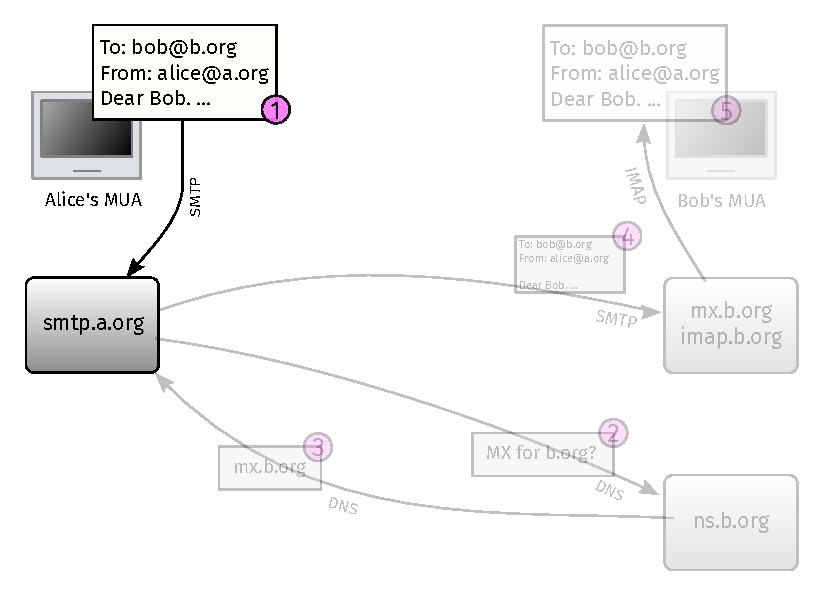
\includegraphics[width=\textwidth]{graphics/Email1.pdf}}
    \only<2>{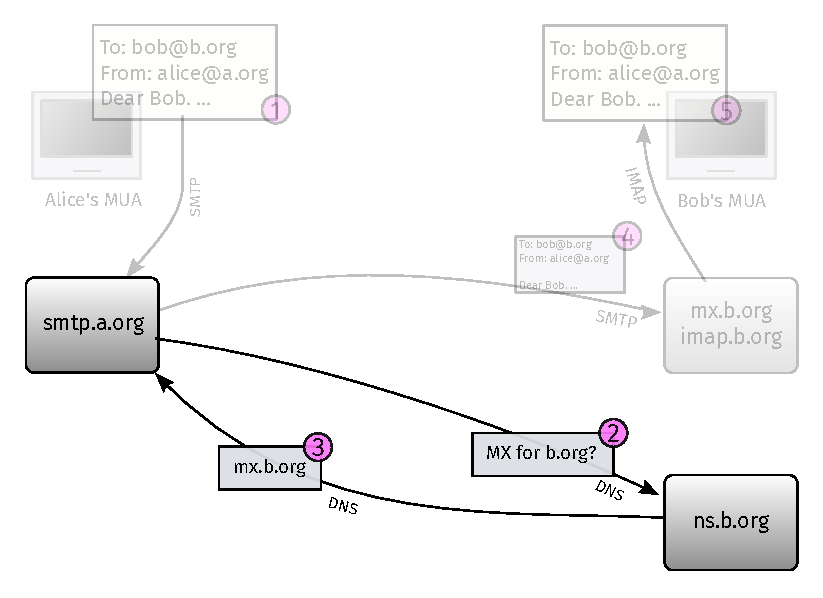
\includegraphics[width=\textwidth]{graphics/Email2.pdf}}
    \only<3>{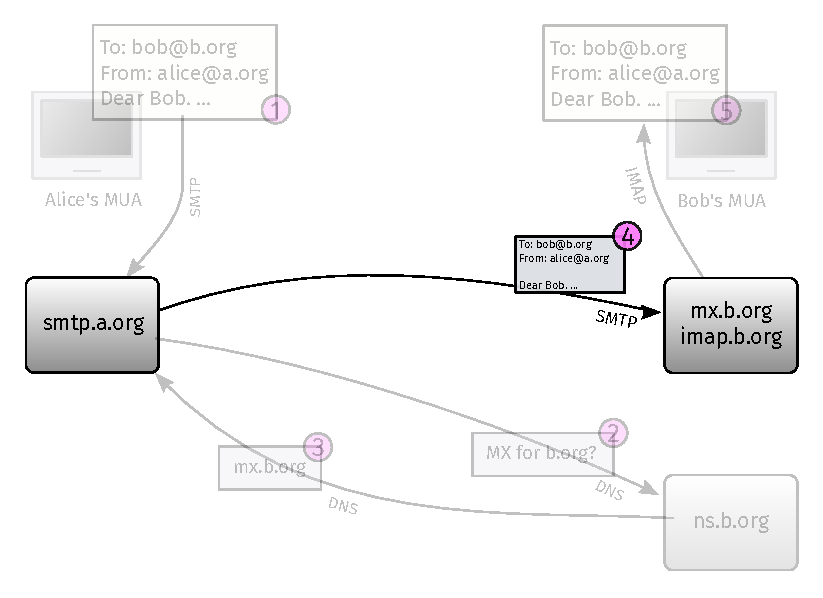
\includegraphics[width=\textwidth]{graphics/Email3.pdf}}
    \only<4>{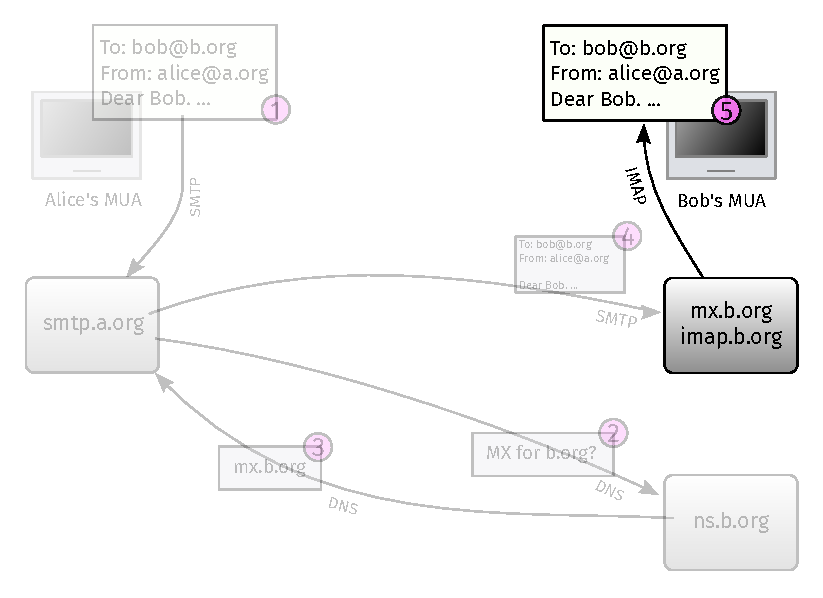
\includegraphics[width=\textwidth]{graphics/Email4.pdf}}
\end{frame}

\begin{frame}{Let's Send an Email (SMTP)}
    \ttfamily
    \footnotesize
    \$ \textbf{telnet smtp.mines.edu 25} \\
    220 izzard.mines.edu ESMTP Sendmail 8.14.4 \\
    \pause
    \textbf{HELO isengard} \\
    250 izzard.mines.edu Hello isengard, pleased to meet you \\
    \pause
    \textbf{MAIL From:jrosenth@mimes.edu} \\
    250 2.1.0 jrosenth@mimes.edu... Sender ok \\
    \pause
    \textbf{RCPT To:rack@josenth.al} \\
    250 2.1.5 rack@josenth.al... Recipient ok \\
    \pause
    \textbf{DATA} \\
    354 Enter mail, end with "." on a line by itself \\
    \pause
    \textbf{Subject: This is my Email \\
    \\
    This is the message body \\
    .} \\
    250 2.0.0 v9J0V6dW022526 Message accepted for delivery \\
    \pause
    \textbf{QUIT} \\
    221 2.0.0 izzard.mines.edu closing connection
\end{frame}

\begin{frame}{What did \texttt{izzard} do?}
    \begin{enumerate}[<+->]
        \item Lookup MX records for \texttt{rosenth.al} (\texttt{po.640k.net})
        \item Connect to \texttt{po.640k.net:25}\dots \\
            \texttt{HELO izzard.mines.edu} \\
            \texttt{MAIL From:jrosenth@mimes.edu} \\
            \texttt{RCPT To:rack@josenth.al} \\
            \dots
    \end{enumerate}
    \pause[\thebeamerpauses]
    \dots{}then the MTA on \texttt{po} hands the message off to the MDA, and
    the MUA downloads the message from the MDA.
\end{frame}

\section{Part 2: Setting Up Your Own Mail Server on Linux}

\begin{frame}{Postfix}
    \begin{center}
        
\includegraphics[width=0.5\textwidth]{graphics/mysza.png}
    \end{center}

    \begin{itemize}[<+->]
        \item Sendmail-compatible MTA
        \item 1998
        \item Knows how to speak LMTP (Local Mail Transport Protocol)
        \item \emph{Does The Job}™
    \end{itemize}
\end{frame}

\begin{frame}{Dovecot}
    \begin{center}
        
\includegraphics[width=0.4\textwidth]{graphics/dovecot}
    \end{center}
    \begin{columns}
        \begin{column}{0.175\textwidth}
        \end{column}
        \begin{column}{0.65\textwidth}
            \begin{itemize}[<+->]
                \item MDA, provides POP3 and IMAP
                \item Stores your mail
                \item Accepts mail by providing LMTP
                \item Filter mail with Pigeonhole Sieve
            \end{itemize}
        \end{column}
        \begin{column}{0.175\textwidth}
        \end{column}
    \end{columns}
\end{frame}

\begin{frame}[fragile]{Configuring Postfix}
    \begin{block}{\ttfamily /etc/postfix/main.cf}
    \begin{minted}{ini}
        myhostname = po.640k.net
        mydomain = po.640k.net

        # what domains to consider ourselves
        mydestination = po.640k.net, localhost

        # listen on all network interfaces
        inet_interfaces = all

        # only allow mail to us or authenticated
        smtpd_relay_restrictions = permit_mynetworks,
            permit_sasl_authenticated,
            reject_unauth_destination
    \end{minted}
    \end{block}
\end{frame}

\begin{frame}[fragile]{Virtual Alias Maps}
    \begin{block}{\ttfamily /etc/postfix/main.cf}
    \begin{minted}{ini}
        # virtual domains should _not_ go
        # under "mydestination"
        virtual_alias_domains = rosenth.al
          steamboatnetworks.net steamboatnetworks.com
        virtual_alias_maps = hash:/etc/postfix/virtual
    \end{minted}
    \end{block}

    \begin{block}{\ttfamily /etc/postfix/virtual}
    \begin{minted}{text}
        rack@josenth.al             jrosenth
        jack@steamboatnotworks.net  jrosenth
        ...
    \end{minted}
    \end{block}

    Then run \verb|# postmap /etc/postfix/virtual|
\end{frame}

\begin{frame}[fragile]{SSL/TLS Thy Postfix}
    Let's Encrypt is my drug of choice: \\
    {\small \verb|# certbot certonly --standalone -d po.640k.net|}
    \pause

    \begin{block}{\ttfamily /etc/postfix/main.cf}
    \begin{minted}[fontsize=\small]{ini}
        smtpd_tls_cert_file=
            /etc/letsencrypt/live/po.640k.net/fullchain.pem
        smtpd_tls_key_file=
            /etc/letsencrypt/live/po.640k.net/privkey.pem
        smtpd_use_tls=yes
    \end{minted}
    \pause
    \begin{minted}[fontsize=\small]{ini}
        # Settings for POODLE and the like
        smtpd_tls_mandatory_protocols=!SSLv2,!SSLv3
        smtp_tls_mandatory_protocols=!SSLv2,!SSLv3
        smtpd_tls_protocols=!SSLv2,!SSLv3
        smtp_tls_protocols=!SSLv2,!SSLv3
    \end{minted}
    \end{block}
\end{frame}

\begin{frame}[fragile]{Postfix Services}
    Uncomment each of the following lines:

    \begin{block}{\ttfamily /etc/postfix/\emph{master}.cf}
    \begin{minted}{ini}
        smtp        inet    n - n - -   smtpd
        submission  inet    n - n - -   smtpd
        smtps       inet    n - n - -   smtpd
         -o smtpd_tls_wrappermode=yes
    \end{minted}
    \end{block}

    \pause
    \bigskip

    If you enable \texttt{smtps} as above, Linux will not know what port to
    put it on. Add to \texttt{/etc/services}: \\
    \verb|smtps         465/tcp|
\end{frame}

\begin{frame}[fragile]{Start and Test Postfix}
    \begin{enumerate}
        \item Start Postfix (change as needed for \texttt{init} systems):
            \begin{minted}{console}
                # systemctl start postfix
            \end{minted}
        \item Send yourself an Email:
            \begin{minted}{console}
                $ fortune | mail jrosenth@mimes.edu
            \end{minted}
    \end{enumerate}
\end{frame}

\begin{frame}[fragile]{Dovecot Setup}
    \begin{enumerate}[<+->]
        \item Copy sample configs from
            \texttt{/usr/share/doc/dovecot/example-config} \\
            to \texttt{/etc/dovecot}

        \item Edit \texttt{/etc/dovecot/dovecot.conf}:
            \begin{minted}[bgcolor=block body.bg]{ini}
                # Protocols we want to be serving
                protocols = imap lmtp
            \end{minted}

        \item \texttt{cd} to \texttt{/etc/dovecot/conf.d} and get ready to edit
            \emph{a lot} of files
    \end{enumerate}
\end{frame}

\begin{frame}[fragile]{Mailbox Storage Format}
    You'll need to decide how you want to store mail:
    \begin{description}[<+->]
        \item[\texttt{mbox}] Traditional UNIX mailbox storage format: one file
            per mailbox.
        \item[\texttt{maildir}] Directories with one file per message.
        \item[\texttt{sdbox}] Dovecot's own high performance storage format
            (one message per file).
        \item[\texttt{mdbox}] Dovecot's own high performance storage format
            (multiple messages per file).
    \end{description}

    \pause[\thebeamerpauses]
    Set your choice in \texttt{10-mail.conf}:
    \begin{minted}[bgcolor=block body.bg]{ini}
        mail_location = mdbox:~/mdbox
    \end{minted}
\end{frame}

\begin{frame}[fragile]{Authentication}
    \begin{block}{\ttfamily 10-auth.conf}
    \begin{minted}{ini}
        # given user@example.com, username is "user"
        auth_username_format = %Ln
    \end{minted}
    \end{block}
    \pause
    \medskip

    Need to ask PAM to let us check:
    \begin{block}{\ttfamily /etc/pam.d/dovecot}
    \begin{minted}{text}
        auth    required    pam_unix.so nullok
        account required    pam_unix.so
    \end{minted}
    \end{block}
\end{frame}

\begin{frame}[fragile]{Wiring-up Auth to Postfix}
    \begin{block}{\ttfamily 10-master.conf}
        \begin{minted}[fontsize=\small]{lighttpd}
            service auth {
              unix_listener /var/spool/postfix/private/auth {
                mode = 0660
                user = postfix
                group = postfix
              }
            }
        \end{minted}
    \end{block}
    \begin{block}{\ttfamily /etc/postfix/main.cf}
        \begin{minted}[fontsize=\small]{ini}
            smtpd_sasl_type = dovecot
            smtpd_sasl_path = private/auth
            smtpd_sasl_auth_enable = yes
        \end{minted}
    \end{block}
\end{frame}

\begin{frame}[fragile]{Wiring-up LMTP to Postfix}
    \begin{block}{\ttfamily 10-master.conf}
        \begin{minted}[fontsize=\small]{lighttpd}
            service lmtp {
              unix_listener /var/spool/postfix/private/lmtp {
                mode = 0660
                user = postfix
                group = postfix
              }
            }
        \end{minted}
    \end{block}
    \begin{block}{\ttfamily /etc/postfix/main.cf}
        \begin{minted}[fontsize=\small]{ini}
            mailbox_transport = lmtp:unix:private/lmtp
        \end{minted}
    \end{block}
\end{frame}

\begin{frame}[fragile]{SSL/TLS in Dovecot}
    \begin{block}{\ttfamily 10-ssl.conf}
        \begin{minted}[fontsize=\small]{ini}
            ssl = required
            ssl_cert =
              </etc/letsencrypt/live/po.640k.net/fullchain.pem
            ssl_key =
              </etc/letsencrypt/live/po.640k.net/privkey.pem
        \end{minted}
    \end{block}
    \pause
    See config files for POODLE settings and the like.
\end{frame}

\begin{frame}[fragile]{Ready, Set, Email!}
    Fire up Dovecot and restart Postfix:
    \begin{minted}{console}
        # systemctl start dovecot
        # systemctl restart postfix
    \end{minted}

    \pause

    Now, \emph{send some test emails}!
\end{frame}

\begin{frame}[standout]
    \Huge
    Questions?
\end{frame}

\end{document}
